\documentclass[a4paper, czech]{article}

\usepackage[czech]{babel}
\usepackage{indentfirst}
\usepackage{graphicx}
\usepackage{float}
\usepackage[margin=1.5cm]{geometry}
\usepackage{booktabs}
\usepackage{amsmath}
\usepackage[table]{xcolor}
\usepackage{multirow}
\usepackage{tabularray}
\usepackage{bold-extra}


\begin{document}
\begin{table}[H]
    \centering
    \begin{tblr}{
        cell{1}{1} = {c = 2, r = 4}{c}, % Logo
        cell{1}{4} = {c = 3}{c}, % Předmět
        cell{2}{4} = {c = 3}{c}, % Jméno
        cell{3}{4} = {}{c}, % Ročník
        cell{3}{6} = {}{c}, % Studijní skupina
        cell{4}{4} = {}{c}, % Spolupracoval
        cell{4}{6} = {}{c}, % Mereno dne
        cell{5}{1} = {c = 2}{55mm}, % Kontroloval
        cell{5}{3} = {c = 2}{55mm}, % Hodnoceni
        cell{5}{5} = {c = 2}{55mm}, % Dne
        cell{6}{2} = {c = 5}{}, % Nazev ulohy
        cell{7}{1} = {}{c}, % Číslo úlohy
        cell{7}{2} = {c = 5}{c}, % Název úlohy
        vline{1,2,7} = {1.2pt},
        vline{3,5},
        hline{1,5,6,8} = {1.2pt},
        hline{2,3,4}
        }
        
\includegraphics{logo_fekt.png} & & \textsuperscript{Předmět} & \large \textbf{Měření v audiotechnice} \\
             & & \textsuperscript{Jméno} & \large \textbf{Karolína Šebestová} \\
             & & \textsuperscript{Ročník} & \large \textbf{3.} & \textsuperscript{Studijní skupina} & \large \textbf{St 14:00} \\
             & & \textsuperscript{Spolupracoval} & \large \textbf{Filip Kokavec} & \textsuperscript{Měřeno dne} & \large \textbf{16.10.2024} \\
        \textsuperscript{Kontroloval} & & \textsuperscript{Hodnocení} & & \textsuperscript{Dne} \\
        \textsuperscript{Číslo úlohy} & \textsuperscript{Název úlohy} \\
        \Large \textbf{3A} & \Large \textsc{\textbf{Měření odporů malých hodnot}} \\
    \end{tblr}
\end{table}

\section{Zadání}

\begin{itemize}
    \item Změřte odpory vzorků srovnávací metodou na automatizovaném pracovišti.
    \item Vypočítejte nejistoty změřených hodnot odporů vodičů.
\end{itemize}

\section{Teoretický úvod}

K měření elektrických odporů o velmi malých hodnotách ($<1 \Omega$) je možné použít například Thomsonův dvojitý můstek, Ohmovu metodu se čtyřsvorkovým zapojením nebo srovnávací metodu v sériovém zapojení.
Přesnost měření dále závisí na přechodových odporech vodivých spojů v měřeném obvodě, odporů přívodů obvodu a termoelektrického napĚtí v obvodě.

\subsection{Srovnávací metoda}

Princip této metody spočívá v měření úbytku napětí na známém odporu (odporovém etalonu) a na neznámém odporu (měřeném vzorku).
Oba odpory jsou zapojeny v sérii, co znamená, že oběma teče stejný konstantní elektrický proud.
Hodnotu neznámého odporu $R_X$ určíme pomocí známé hodnoty odporového etalonu $R_N$ a poměru úbytku napětí dle vztahu:

\begin{equation*}
    R_X = \frac{U_X}{U_N} \cdot R_N
\end{equation*}

Relativní odchylka metody $\delta_{R_X}$ je:

\begin{equation*}
    \delta_{R_X} = \left|\frac{R_N - R_X}{R_X + R_V}\right| \cdot 100 \%
\end{equation*}

$R_V$ je hodnota vnitřního odporu voltmetru.

Pro minimalizaci odchylky metody zpúsobené vlivem odporů vodičů a svorek se používá čtyřsvorkové zapojení vzorku i etalonu.
Spotřeba přístroje se zanedbává, protože má poměrně velký vstupní odpor.
Pro odstranění vlivu termoelektrického napětí v obvodě se měří při obou polaritách elektrického proudu.
Nejistota měření je minimalizována vícenásobným měřením a použitím přesných částí měřeného obvodu.
Místo napětí $U_X$ a $U_N$ proto ve vztahu používáme jejich odhady (průměry) $\bar{U}_X$ a $\bar{U}_N$.

Nejistotu odhadu odporu $\bar{U}_N$ určíme vztahem:
\begin{equation*}
    u_{\bar{R}_X} = \sqrt{\left( \frac{\bar{U}_X}{\bar{U}_N} \cdot u_{BR_N} \right)^2 + \left( \frac{R_N}{\bar{U}_N} \cdot u_{CU_X} \right)^2 + \left( \frac{\bar{U}_X \cdot R_N}{\bar{U}_N^2} \cdot u_{CU_N} \right)^2 - 2 \cdot \frac{\bar{U}_X \cdot R_N^2}{\bar{U}_N^3} \cdot u_{CU_X} \cdot u_{CU_N}}
\end{equation*}
kde $\bar{U}_X$ a $\bar{U}_N$ jsou střední hodnoty napětí na odporech, $R_X$ a $R_N$ jsou hodnoty normálového měřeného odporu, $u_{BR_N}$ je standardní nejistota odporu etalonu, $u_{CU_N}$ a $u_{CU_X}$ jsou standardní kombinovanou nejistotou voltmetru.

\begin{figure}[H]
    \centering
    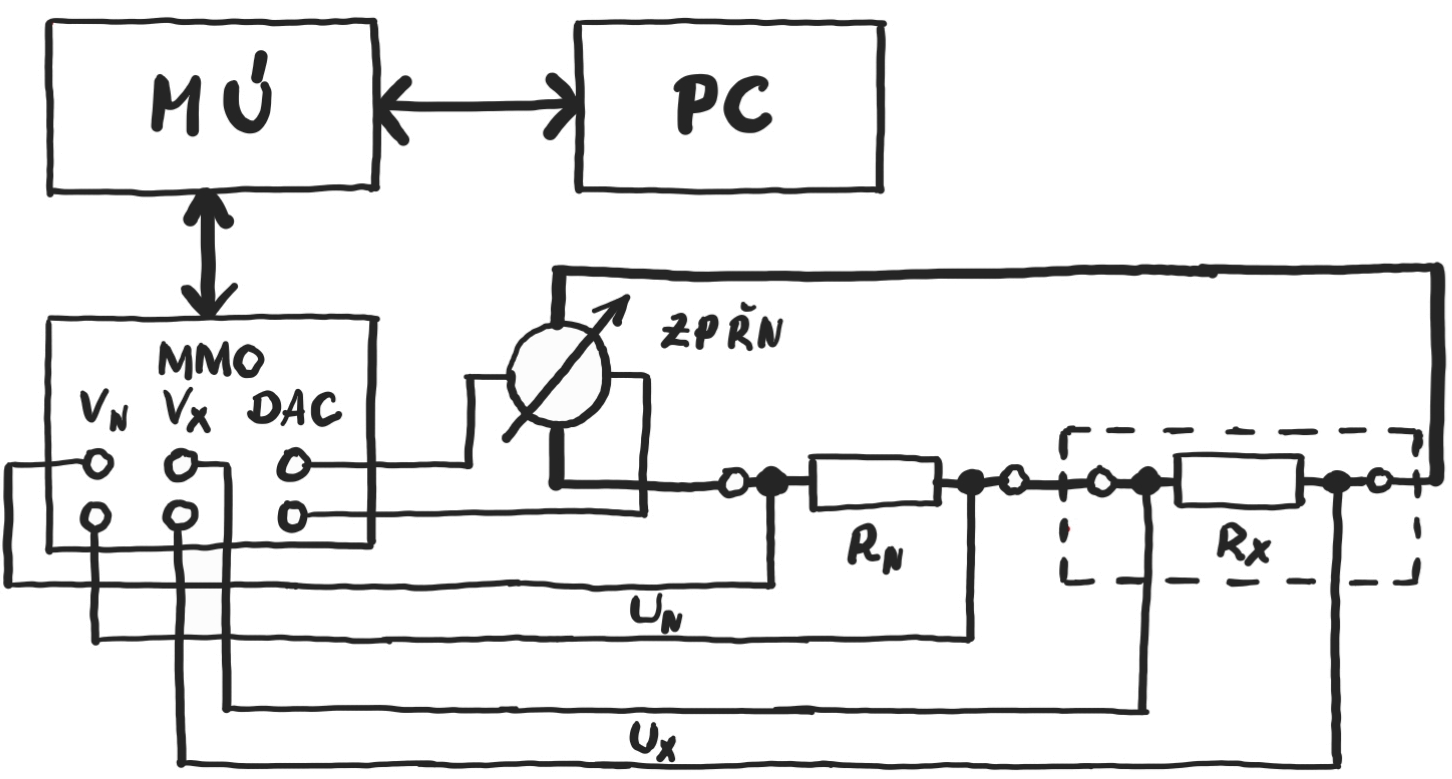
\includegraphics[width=0.6\textwidth]{schema3a.png}
    \caption{Schéma zapojení pro automatické měření}
\end{figure}

\section{Výsledky měření}

\subsection{Tabulky}

\begin{table}[H]
    \centering
    \caption{Automatizované měření odporu hliníkového vzorku}
    \begin{tabular}{>{\columncolor{cyan!20}}c>{\columncolor{cyan!20}}c>{\columncolor{cyan!20}}c>{\columncolor{cyan!20}}ccccc}
        \hline
        \rowcolor{cyan} Měření & $U_X$ {[}V{]} & $U_N$ {[}V{]} & $R_X$ {[}$\Omega${]} & $\delta_{U_X}'$ {[}\%{]} & $\delta_{U_N}'$ {[}\%{]} & $u_{BU_X}'$ {[}V{]} & $u_{BU_N}'$ {[}V{]} \\
        \hline
        1      & 3,253E-05  & 1,713E-05  & 1,899E-03    & 0,25          & 0,38          & 2,310E-06     & 2,310E-06     \\
        2      & 3,286E-05  & 1,697E-05  & 1,936E-03    & 1,25          & 1,32          & 2,310E-06     & 2,310E-06     \\
        3      & 3,221E-05  & 1,713E-05  & 1,880E-03    & 0,75          & 0,38          & 2,310E-06     & 2,310E-06     \\
        4      & 3,275E-05  & 1,724E-05  & 1,899E-03    & 0,92          & 0,25          & 2,310E-06     & 2,310E-06     \\
        5      & 3,242E-05  & 1,746E-05  & 1,857E-03    & 0,08          & 1,51          & 2,310E-06     & 2,310E-06     \\
        6      & 3,280E-05  & 1,686E-05  & 1,945E-03    & 1,09          & 1,95          & 2,310E-06     & 2,310E-06     \\
        7      & 3,221E-05  & 1,713E-05  & 1,880E-03    & 0,75          & 0,38          & 2,310E-06     & 2,310E-06     \\
        8      & 3,226E-05  & 1,735E-05  & 1,859E-03    & 0,58          & 0,88          & 2,310E-06     & 2,310E-06     \\
        9      & 3,237E-05  & 1,735E-05  & 1,866E-03    & 0,25          & 0,88          & 2,310E-06     & 2,310E-06     \\
        10     & 3,210E-05  & 1,735E-05  & 1,850E-03    & 1,09          & 0,88          & 2,310E-06     & 2,310E-06 \\
        \hline
    \end{tabular}

    \begin{tabular}{cc}
        \hline
        \cellcolor{lightgray}    Počet měření                     & \cellcolor{blue!30} 10         \\
        \cellcolor{lightgray} Materiál vodiče                       & \cellcolor{blue!30} hliník     \\
        \cellcolor{lightgray} Průměr vodiče $D_X$ {[}m{]}              & \cellcolor{blue!30} 0,0029     \\
        \cellcolor{lightgray} Délka měřené části vodiče l {[}m{]}   & \cellcolor{blue!30} 0,485      \\
        \cellcolor{lightgray} Odpor etalonu {[}W{]}                 & \cellcolor{blue!30} 0,001      \\
        \cellcolor{lightgray} Tolerance etalonu $\delta_{R_N}$ {[}\%{]}        & \cellcolor{blue!30} 0,010      \\
        Standarní nejistota $u_{BR_N}$ {[}V{]}      & 5,7735E-08 \\
        Odpor měřeného vodiče $R_X$ {[}W{]}      & 1,887E-03        \\
        $\delta_{R_X}$ {[}\%{]}                          & 30,73        \\
        $\delta_{U_X}$ {[}\%{]}                          & 0,70        \\
        $\delta_{U_N}$ {[}\%{]}                          & 0,88        \\
        $u_{BU_X}$ {[}V{]}                          & 2,310E-06        \\
        $u_{BU_N}$ {[}V{]}                          & 2,310E-06        \\
        $u_{AU_X}$ {[}V{]}                          & 8,642E-08        \\
        $u_{AU_N}$ {[}V{]}                          & 5,927E-08        \\
        $u_{CU_X}$ {[}V{]}                          & 2,312E-06        \\
        $u_{CU_N}$ {[}V{]}                          & 2,311E-06        \\
        \cellcolor{lightgray} $u_{R_X}$ [$\mu \Omega$]                          & \cellcolor{blue!30} 119,0724     \\
        \cellcolor{lightgray} $\tilde{U}_{R_X}$ [\%]                     & \cellcolor{blue!30} 12,619         \\
        \cellcolor{lightgray} $R_X$ [$m \Omega$]                  & \cellcolor{blue!30} 1,8871            \\
        \cellcolor{lightgray} $\rho_X$ [$\mu \Omega \cdot m$]                       & \cellcolor{blue!30} 0,0257    \\
        \hline
    \end{tabular}
\end{table}

\begin{table}[H]
    \centering
    \caption{Automatizované měření odporu měděného vzorku}
    \begin{tabular}{>{\columncolor{orange!20}}c>{\columncolor{orange!20}}c>{\columncolor{orange!20}}c>{\columncolor{orange!20}}ccccc}
        \hline
        \rowcolor{yellow} Měření & $U_X$ {[}V{]} & $U_N$ {[}V{]} & $R_X$ {[}$\Omega${]} & $\delta_{U_X}'$ {[}\%{]} & $\delta_{U_N}'$ {[}\%{]} & $u_{BU_X}'$ {[}V{]} & $u_{BU_N}'$ {[}V{]} \\
        \hline
        1  & 1,442E-05 & 8,404E-06 & 1,716E-03 & 5,34 & 1,71 & 2,310E-06 & 2,310E-06 \\
        2  & 1,496E-05 & 8,676E-06 & 1,725E-03 & 1,78 & 1,46 & 2,310E-06 & 2,310E-06 \\
        3  & 1,513E-05 & 8,458E-06 & 1,789E-03 & 0,71 & 1,08 & 2,310E-06 & 2,310E-06 \\
        4  & 1,513E-05 & 8,079E-06 & 1,872E-03 & 0,71 & 5,51 & 2,310E-06 & 2,310E-06 \\
        5  & 1,545E-05 & 8,458E-06 & 1,827E-03 & 1,42 & 1,08 & 2,310E-06 & 2,310E-06 \\
        6  & 1,529E-05 & 9,001E-06 & 1,699E-03 & 0,36 & 5,26 & 2,310E-06 & 2,310E-06 \\
        7  & 1,551E-05 & 8,513E-06 & 1,822E-03 & 1,78 & 0,44 & 2,310E-06 & 2,310E-06 \\
        8  & 1,534E-05 & 8,729E-06 & 1,758E-03 & 0,71 & 2,09 & 2,310E-06 & 2,310E-06 \\
        9  & 1,572E-05 & 8,621E-06 & 1,824E-03 & 3,20 & 0,83 & 2,310E-06 & 2,310E-06 \\
        10 & 1,540E-05 & 8,567E-06 & 1,798E-03 & 1,07 & 0,19 & 2,310E-06 & 2,310E-06 \\
        \hline
    \end{tabular}

    \begin{tabular}{cc}
        \hline
        \cellcolor{lightgray}    Počet měření                     & \cellcolor{yellow} 10         \\
        \cellcolor{lightgray} Materiál vodiče                       & \cellcolor{yellow} měď    \\
        \cellcolor{lightgray} Průměr vodiče $D_X$ {[}m{]}              & \cellcolor{yellow} 0,00275     \\
        \cellcolor{lightgray} Délka měřené části vodiče l {[}m{]}   & \cellcolor{yellow} 0,485      \\
        \cellcolor{lightgray} Odpor etalonu {[}W{]}                 & \cellcolor{yellow} 0,001      \\
        \cellcolor{lightgray} Tolerance etalonu $\delta_{R_N}$ {[}\%{]}        & \cellcolor{yellow} 0,010      \\
        Standarní nejistota $u_{BR_N}$ {[}V{]}      & 5,7735E-08 \\
        Odpor měřeného vodiče $R_X$ {[}W{]}      & 1,783E-03  \\
        $\delta_{R_X}$ {[}\%{]}                          & 28,13      \\
        $\delta_{U_X}$ {[}\%{]}                          & 1,71       \\
        $\delta_{U_N}$ {[}\%{]}                          & 1,97       \\
        $u_{BU_X}$ {[}V{]}                          & 2,310E-06  \\
        $u_{BU_N}$ {[}V{]}                          & 2,310E-06  \\
        $u_{AU_X}$ {[}V{]}                          & 1,134E-07  \\
        $u_{AU_N}$ {[}V{]}                          & 7,583E-08  \\
        $u_{CU_X}$ {[}V{]}                          & 2,313E-06  \\
        $u_{CU_N}$ {[}V{]}                          & 2,311E-06  \\
        \cellcolor{lightgray} $u_{R_X}$ [$\mu \Omega$]                          & \cellcolor{yellow} 211,1112   \\
        \cellcolor{lightgray} $\tilde{U}_{R_X}$ [\%]                     & \cellcolor{yellow} 23,682     \\
        \cellcolor{lightgray} $R_X$ [$m \Omega$]                  & \cellcolor{yellow} 1,7829     \\
        \cellcolor{lightgray} $\rho_X$ [$\mu \Omega \cdot m$]                       & \cellcolor{yellow} 0,0218      \\
        \hline
    \end{tabular}
\end{table}

\begin{table}[H]
    \centering
    \caption{Automatizované měření odporu ocelového vzorku}
    \begin{tabular}{>{\columncolor{lightgray!50}}c>{\columncolor{lightgray!50}}c>{\columncolor{lightgray!50}}c>{\columncolor{lightgray!50}}ccccc}
        \hline
        \rowcolor{lightgray} Měření & $U_X$ {[}V{]} & $U_N$ {[}V{]} & $R_X$ {[}$\Omega${]} & $\delta_{U_X}'$ {[}\%{]} & $\delta_{U_N}'$ {[}\%{]} & $u_{BU_X}'$ {[}V{]} & $u_{BU_N}'$ {[}V{]} \\
        \hline
        1  & 7,987E-05 & 8,405E-06 & 9,503E-03 & 2,32 & 4,02 & 2,312E-06 & 2,310E-06 \\
        2  & 8,100E-05 & 8,838E-06 & 9,165E-03 & 0,93 & 0,93 & 2,312E-06 & 2,310E-06 \\
        3  & 8,182E-05 & 8,947E-06 & 9,145E-03 & 0,07 & 2,17 & 2,312E-06 & 2,310E-06 \\
        4  & 8,182E-05 & 9,055E-06 & 9,036E-03 & 0,07 & 3,41 & 2,312E-06 & 2,310E-06 \\
        5  & 8,220E-05 & 8,946E-06 & 9,188E-03 & 0,53 & 2,16 & 2,312E-06 & 2,310E-06 \\
        6  & 8,171E-05 & 8,838E-06 & 9,245E-03 & 0,07 & 0,93 & 2,312E-06 & 2,310E-06 \\
        7  & 8,236E-05 & 8,405E-06 & 9,800E-03 & 0,73 & 4,02 & 2,312E-06 & 2,310E-06 \\
        8  & 8,225E-05 & 8,784E-06 & 9,364E-03 & 0,60 & 0,31 & 2,312E-06 & 2,310E-06 \\
        9  & 8,214E-05 & 8,350E-06 & 9,837E-03 & 0,46 & 4,64 & 2,312E-06 & 2,310E-06 \\
        10 & 8,247E-05 & 9,001E-06 & 9,163E-03 & 0,86 & 2,78 & 2,312E-06 & 2,310E-06 \\
        \hline
    \end{tabular}

    \begin{tabular}{cc}
        \hline
        \cellcolor{lightgray}    Počet měření                     & \cellcolor{lightgray!50} 10         \\
        \cellcolor{lightgray} Materiál vodiče                       & \cellcolor{lightgray!50} železo     \\
        \cellcolor{lightgray} Průměr vodiče $D_X$ {[}m{]}              & \cellcolor{lightgray!50} 0,0031     \\
        \cellcolor{lightgray} Délka měřené části vodiče l {[}m{]}   & \cellcolor{lightgray!50} 0,485      \\
        \cellcolor{lightgray} Odpor etalonu {[}W{]}                 & \cellcolor{lightgray!50} 0,001      \\
        \cellcolor{lightgray} Tolerance etalonu $\delta_{R_N}$ {[}\%{]}        & \cellcolor{lightgray!50} 0,010      \\
        Standarní nejistota $u_{BR_N}$ {[}V{]}      & 5,7735E-08 \\
        Odpor měřeného vodiče $R_X$ {[}W{]}      & 9,345E-03  \\
        $\delta_{R_X}$ {[}\%{]}                          & 80,67      \\
        $\delta_{U_X}$ {[}\%{]}                          & 0,66       \\
        $\delta_{U_N}$ {[}\%{]}                          & 2,54       \\
        $u_{BU_X}$ {[}V{]}                          & 2,312E-06  \\
        $u_{BU_N}$ {[}V{]}                          & 2,310E-06  \\
        $u_{AU_X}$ {[}V{]}                          & 2,497E-07  \\
        $u_{AU_N}$ {[}V{]}                          & 8,483E-08  \\
        $u_{CU_X}$ {[}V{]}                          & 2,325E-06  \\
        $u_{CU_N}$ {[}V{]}                          & 2,311E-06  \\
        \cellcolor{lightgray} $u_{R_X}$ [$\mu \Omega$]                          & \cellcolor{lightgray!50} 2198,9307  \\
        \cellcolor{lightgray} $\tilde{U}_{R_X}$ [\%]                     & \cellcolor{lightgray!50} 47,063     \\
        \cellcolor{lightgray} $R_X$ [$m \Omega$]                  & \cellcolor{lightgray!50} 9,3446     \\
        \cellcolor{lightgray} $\rho_X$ [$\mu \Omega \cdot m$]                       & \cellcolor{lightgray!50} 0,1454       \\
        \hline
    \end{tabular}
\end{table}

\begin{table}[H]
    \centering
    \caption{Automatizované měření odporu mosazného vzorku}
    \begin{tabular}{>{\columncolor{yellow!35}}c>{\columncolor{yellow!35}}c>{\columncolor{yellow!35}}c>{\columncolor{yellow!35}}ccccc}
        \hline
        \rowcolor{yellow} Měření & $U_X$ {[}V{]} & $U_N$ {[}V{]} & $R_X$ {[}$\Omega${]} & $\delta_{U_X}'$ {[}\%{]} & $\delta_{U_N}'$ {[}\%{]} & $u_{BU_X}'$ {[}V{]} & $u_{BU_N}'$ {[}V{]} \\
        \hline
        1  & 5,774E-05 & 8,133E-06 & 7,100E-03 & 3,15 & 3,97 & 2,311E-06 & 2,310E-06 \\
        2  & 5,872E-05 & 8,567E-06 & 6,854E-03 & 1,51 & 1,15 & 2,311E-06 & 2,310E-06 \\
        3  & 5,959E-05 & 8,513E-06 & 7,000E-03 & 0,05 & 0,51 & 2,311E-06 & 2,310E-06 \\
        4  & 5,991E-05 & 8,242E-06 & 7,270E-03 & 0,49 & 2,69 & 2,311E-06 & 2,310E-06 \\
        5  & 5,937E-05 & 8,296E-06 & 7,157E-03 & 0,42 & 2,05 & 2,311E-06 & 2,310E-06 \\
        6  & 6,002E-05 & 8,513E-06 & 7,051E-03 & 0,67 & 0,51 & 2,311E-06 & 2,310E-06 \\
        7  & 6,008E-05 & 8,296E-06 & 7,242E-03 & 0,76 & 2,05 & 2,311E-06 & 2,310E-06 \\
        8  & 6,024E-05 & 8,459E-06 & 7,122E-03 & 1,04 & 0,13 & 2,311E-06 & 2,310E-06 \\
        9  & 6,040E-05 & 8,675E-06 & 6,963E-03 & 1,31 & 2,43 & 2,311E-06 & 2,310E-06 \\
        10 & 6,013E-05 & 9,001E-06 & 6,681E-03 & 0,85 & 6,27 & 2,311E-06 & 2,310E-06 \\
        \hline
    \end{tabular}

    \begin{tabular}{cc}
        \hline
        \cellcolor{lightgray}    Počet měření                     & \cellcolor{yellow!35} 10         \\
        \cellcolor{lightgray} Materiál vodiče                       & \cellcolor{yellow!35} mosaz      \\
        \cellcolor{lightgray} Průměr vodiče $D_X$ {[}m{]}              & \cellcolor{yellow!35} 0,0026     \\
        \cellcolor{lightgray} Délka měřené části vodiče l {[}m{]}   & \cellcolor{yellow!35} 0,485      \\
        \cellcolor{lightgray} Odpor etalonu {[}W{]}                 & \cellcolor{yellow!35} 0,001      \\
        \cellcolor{lightgray} Tolerance etalonu $\delta_{R_N}$ {[}\%{]}        & \cellcolor{yellow!35} 0,010      \\
        Standarní nejistota $u_{BR_N}$ {[}V{]}      & 5,7735E-08 \\
        Odpor měřeného vodiče $R_X$ {[}W{]}      & 7,044E-03  \\
        $\delta_{R_X}$ {[}\%{]}                          & 75,14      \\
        $\delta_{U_X}$ {[}\%{]}                          & 1,03       \\
        $\delta_{U_N}$ {[}\%{]}                          & 2,18       \\
        $u_{BU_X}$ {[}V{]}                          & 2,311E-06  \\
        $u_{BU_N}$ {[}V{]}                          & 2,310E-06  \\
        $u_{AU_X}$ {[}V{]}                          & 2,603E-07  \\
        $u_{AU_N}$ {[}V{]}                          & 7,910E-08  \\
        $u_{CU_X}$ {[}V{]}                          & 2,326E-06  \\
        $u_{CU_N}$ {[}V{]}                          & 2,311E-06  \\
        \cellcolor{lightgray} $u_{R_X}$ [$\mu \Omega$]                          & \cellcolor{yellow!35} 1646,3030  \\
        \cellcolor{lightgray} $\tilde{U}_{R_X}$ [\%]                     & \cellcolor{yellow!35} 46,745     \\
        \cellcolor{lightgray} $R_X$ [$m \Omega$]                  & \cellcolor{yellow!35} 7,0438     \\
        \cellcolor{lightgray} $\rho_X$ [$\mu \Omega \cdot m$]                       & \cellcolor{yellow!35} 0,0771        \\
        \hline
    \end{tabular}
\end{table}

\begin{table}[H]
    \catcode`\-=12
    \centering
    \caption{Výsledky měření malých odporů}
    \begin{tabular}{ccccccccc}
        \toprule
        \multirow{2}{*}{vzorek} & $D_X$   & $\bar{U}_X$        & $\bar{U}_X$        & $R_X$    & $u_{R_X}$    & $\tilde{U}_{R_X}$   & $\rho_X$     & $\rho_{X_{tab}}$   \\
        \cmidrule{2-9}
                                & mm   & V         & V         & $m \Omega$  & $\mu \Omega$   & \%    & $\mu \Omega \cdot m$ &    $\mu \Omega \cdot m$     \\
        \midrule
        hliník                  & 2,9  & 3,245E-05 & 1,720E-05 & 1,887 & 119,1  & 12,62 & 0,0257 & 0,027   \\
        měď                     & 2,75 & 1,524E-05 & 8,550E-06 & 1,783 & 211,1  & 23,68 & 0,0218 & 0,0178  \\
        ocel                    & 3,1  & 8,176E-05 & 8,757E-06 & 9,345 & 2198,9 & 47,06 & 0,1454 & 0,1-0,2 \\
        mosaz                   & 2,6  & 5,962E-05 & 8,469E-06 & 7,044 & 1646,3 & 46,74 & 0,0771 & 0,08 \\
        \bottomrule
    \end{tabular}
\end{table}

\break

\subsection{Příklady výpočtu}

\begin{enumerate}
    \item Hodnota neznámého odporu $R_X$
    \begin{multline*}
        R_X = \textcolor{teal}{\frac{U_X}{U_N} \cdot R_N} = \frac{3,253 \cdot 10^{-5} V}{1,713 \cdot 10^{-5} V} \cdot 0,001 \Omega = 1,899 \cdot 10 ^{-3} \Omega = \underline{\underline{1,899\ m\Omega}} \hfill
    \end{multline*}

    \item Odhady (střední hodnoty) napětí
    \begin{multline*}
        \bar{U}_X = \frac{U_{X_1} + U_{X_2} + ... + U_{X_{10}}}{10} = 3,245 \cdot 10^{-5} V = \underline{\underline{32,45\ \mu V}} \hfill
    \end{multline*}
    \begin{multline*}
        \bar{U}_N = \frac{U_{N_1} + U_{N_2} + ... + U_{N_{10}}}{10} = 1,720 \cdot 10^{-5} V = \underline{\underline{17,2\ \mu V}} \hfill
    \end{multline*}

    \item Standardní nejistota (typu B) odporu etalonu
    \begin{multline*}
        u_{BR_N} = \textcolor{teal}{\frac{\delta_X \cdot X}{100 \cdot \chi}} = \frac{\delta_{R_N} \cdot R_N}{100 \cdot \chi} = \frac{0,01\% \cdot 0,001 \Omega}{100 \cdot \sqrt{3}} = 57,73 \cdot 10^{-9} \Omega = \underline{\underline{57,73\ n \Omega}} \hfill
    \end{multline*}

    \item Standardní nejistota odporu $\bar{R}_X$
    \begin{multline*}
        u_{\bar{R}_X} = \textcolor{teal}{\sqrt{\left( \frac{\bar{U}_X}{\bar{U}_N} \cdot u_{BR_N} \right)^2 + \left( \frac{R_N}{\bar{U}_N} \cdot u_{CU_X} \right)^2 + \left( \frac{\bar{U}_X \cdot R_N}{\bar{U}_N^2} \cdot u_{CU_N} \right)^2 - 2 \cdot \frac{\bar{U}_X \cdot R_N^2}{\bar{U}_N^3} \cdot u_{CU_X} \cdot u_{CU_N}}} = \\
        = \sqrt{\left( \frac{3,245 \cdot 10^{-5} V}{1,720 \cdot 10^{-5} V} \cdot 57,73 \cdot 10^{-9} \Omega \right)^2 + \left( \frac{0,001 \Omega}{1,720 \cdot 10^{-5} V} \cdot 2,321 \cdot 10^{-6} V \right)^2 +} \\
        \overline{+ \left( \frac{3,245 \cdot 10^{-5} V \cdot 0,001 \Omega}{(1,720 \cdot 10^{-5} V)^2} \cdot 2,311 \cdot 10^{-6} V \right)^2 - 2 \cdot \frac{3,245 \cdot 10^{-5} V \cdot (0,001 \Omega)^2}{(1,720 \cdot 10^{-5} V)^3} \cdot 2,321 \cdot 10^{-6} V \cdot 2,311 \cdot 10^{-6} V } = \\
        = 119,0724 \cdot 10^{-6} \Omega = \underline{\underline{119,0724\ \mu \Omega}}
    \end{multline*}

    \item Relativní rozšířená nejistota
    \begin{multline*}
        \tilde{U}_{R_X} = \frac{k_r \cdot u_{\bar{R}_X}}{R_X} \cdot 100 \% = \frac{2 \cdot 119,0724 \cdot 10^{-6} \Omega}{1,8871 \cdot 10^{-3} \Omega} \cdot 100 \% = \underline{\underline{12,619\ \%}} \hfill
    \end{multline*}

    \item Měrný elektrický odpor
    \begin{multline*}
        \rho_X = \textcolor{teal}{\frac{R_X \cdot S_{Al}}{4 \cdot l}} = \frac{1,8871 \cdot 10^{-3} \Omega \cdot \pi \cdot (0,0029m)^2}{4 \cdot 0,485m} = 0,0257 \cdot 10^{-6} \Omega \cdot m = \underline{\underline{0,0257\ \mu \Omega \cdot m}} \hfill
    \end{multline*}
\end{enumerate}

\section{Seznam použitých přístrojů}

\begin{itemize}
    \item Měřící ústředna Agilent 34972A, v.č. MY49008999
    \item Odporový etalon Metra 0,001$\Omega$ abs., v.č. 5520202
    \item Zdroj proudu řízený napětím ZPŘN
    \item Laboratorní přípravek Měření malých odporů MMO
\end{itemize}

\section{Závěr}

Tímto měřením jsme pomocí srovnávací metody na automatizovaném měrícím pracovišti určili velikosti odporů několika vzorků zkonstruovaných z různých kovových materiálů (hliník, měď, ocel a mosaz).
Následným výpočtem jsme byli schopni určit měrný elektrický odpor materiálů, ze kterých byly vzorky zhotoveny.

Námi vypočtené měrné elektrické odpory hliníku, oceli a mosaze zhruba odpovídají tabulkovým hodnotám.
Hodnota měrného elektrického odporu mědi nám však vyšla podstatně vyšší než tabulková hodnota.
Tento jev je možné vysvětlit různými parazitními jevy uvnitř obvodu, kontaktním odporem na svorkách přípravků, korozí nebo nečistotě na vzorku, případně nesprávným uchycením vzorku do přípravku.

\end{document}